Dans un examen, une épreuve notée sur dix points est constituée de deux exercices : le premier est noté sur deux points, le deuxième sur huit points.


\medskip

\noindent {\Large \textbf{Partie 1}}

\medskip

Le premier exercice est constitué de deux questions Q1 et Q2.

Chaque question est notée sur un point. Une réponse correcte rapporte un point; une réponse incorrecte, incomplète ou une absence de réponse rapporte zéro point.

On considère que :

\begin{itemize}
\item Un candidat pris au hasard a une probabilité 0,8 de répondre correctement à la question Q1.
\item Si le candidat répond correctement à $Q 1$, il a une probabilité 0,6 de répondre correctement à $\mathrm{Q} 2$; s'il ne répond pas correctement à $\mathrm{Q} 1$, il a une probabilité 0,1 de répondre correctement à Q2.
\end{itemize}

On prend un candidat au hasard et on note :

	\begin{itemize}
		\item $A$ l'évènement : \og{}le candidat répond correctement à la question $\mathrm{Q} 1$ \fg{} ;
		\item $B$ l'évènement : \og{}le candidat répond correctement à la question Q2 \fg{}.
	\end{itemize}

On note $\overline{A}$ et $\overline{B}$ les évènements contraires de $A$ et de $B$.

	\begin{enumerate}
		\item Recopier et compléter les pointillés de l'arbre pondéré ci-dessous.

\begin{center}
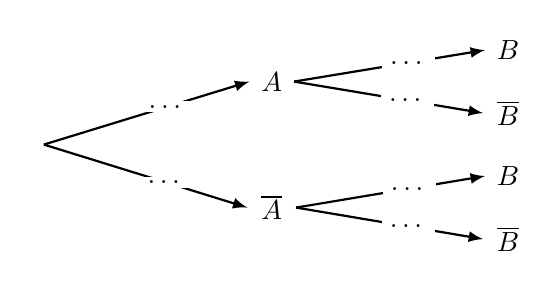
\begin{tikzpicture}[xscale = 1,yscale = 1,baseline = {(R.base)}]
			
			\tikzstyle{fleche} = [->,> = latex,thick]
			\tikzstyle{noeud} = [fill = white,circle,inner sep = 2pt]
			\tikzstyle{feuille} = [fill = white,circle,inner sep = 2pt]
			\tikzstyle{etiquette} = [pos = 0.6,fill = white, inner xsep = 3pt, inner ysep = 1.5pt]
			
			\def\DistanceInterNiveaux{3}
			\def\DistanceInterFeuilles{0.8}
			
			\def\NiveauA{(0)*\DistanceInterNiveaux}
			\def\NiveauB{(1)*\DistanceInterNiveaux}
			\def\NiveauC{(2)*\DistanceInterNiveaux}
			\def\InterFeuilles{(-1)*\DistanceInterFeuilles}
			
			\node[noeud] (R) at ({\NiveauA},{(1.5)*\InterFeuilles}) {};
			\node[noeud] (Ra) at ({\NiveauB},{(0.5)*\InterFeuilles}) {$A$};
			\node[feuille] (Raa) at ({\NiveauC},{(0)*\InterFeuilles}) {$B$};
			\node[feuille] (Rab) at ({\NiveauC},{(1)*\InterFeuilles}) {$\overline{B}$};
			\node[noeud] (Rb) at ({\NiveauB},{(2.5)*\InterFeuilles}) {$\overline{A}$};
			\node[feuille] (Rba) at ({\NiveauC},{(2)*\InterFeuilles}) {$B$};
			\node[feuille] (Rbb) at ({\NiveauC},{(3)*\InterFeuilles}) {$\overline{B}$};
			
			\draw[fleche] (R.east)--(Ra.west) node[etiquette] {\dots};
			\draw[fleche] (Ra.east)--(Raa.west) node[etiquette] {\dots};
			\draw[fleche] (Ra.east)--(Rab.west) node[etiquette] {\dots};
			\draw[fleche] (R.east)--(Rb.west) node[etiquette] {\dots};
			\draw[fleche] (Rb.east)--(Rba.west) node[etiquette] {\dots};
			\draw[fleche] (Rb.east)--(Rbb.west) node[etiquette] {\dots};
\end{tikzpicture}
\end{center}

		\item Calculer la probabilité que le candidat réponde correctement aux deux questions Q1 et Q2.
		\item Calculer la probabilité que le candidat réponde correctement à la question Q2.
	\end{enumerate}

On note :

\begin{itemize}
		\item $X_{1}$ la variable aléatoire qui, à un candidat, associe sa note à la question Q1 ;
		\item $X_{2}$ la variable aléatoire qui, à un candidat, associe sa note à la question Q2 ;
		\item $X$ la variable aléatoire qui, à un candidat, associe sa note à l'exercice, c'est-à-dire $X = X_{1} + X_{2}$.
\end{itemize}

\begin{enumerate}
\setcounter{enumi}{3}
\item Déterminer l'espérance de $X_{1}$ et de $X_{2}$. En déduire l'espérance de $X$. Donner une interprétation de l'espérance de $X$ dans le contexte de l'exercice.

\item On souhaite déterminer la variance de $X$.

	\begin{enumerate}
		\item Déterminer $P(X = 0)$ et $P(X = 2)$. En déduire $P(X = 1)$.

		\item Montrer que la variance de $X$ vaut 0,57 .

		\item A-t-on $V(X) = V\left(X_{1}\right) + V\left(X_{2}\right)$ ? Est-ce surprenant?
	\end{enumerate}
\end{enumerate}


\medskip

\noindent {\Large \textbf{Partie 2}}

\medskip

Le deuxième exercice est constitué de huit questions indépendantes.

Chaque question est notée sur un point. Une réponse correcte rapporte un point ; une réponse incorrecte et une absence de réponse rapporte zéro point.

Les huit questions sont de même difficulté : pour chacune des questions, un candidat a une probabilité $\dfrac{3}{4}$ de répondre correctement, indépendamment des autres questions.

On note $Y$ la variable aléatoire qui, à un candidat, associe sa note au deuxième exercice, c'est-à-dire le nombre de bonnes réponses.

\begin{enumerate}
\item Justifier que $Y$ suit une loi binomiale dont on précisera les paramètres.

\item Donner la valeur exacte de $P(Y = 8)$.

\item Donner l'espérance et la variance de $Y$.

\end{enumerate}


\medskip

\noindent {\Large \textbf{Partie 3}}

\medskip

On suppose que les deux variables aléatoires $X$ et $Y$ sont indépendantes. On note la variable aléatoire qui, à un candidat, associe sa note totale à l'examen : $Z = X + Y$.

\begin{enumerate}
\item Calculer l'espérance et la variance de $Z$.

\item Soit $n$ un nombre entier strictement positif.

Pour $i$ entier variant de 1 à $n$, on note $Z_{i}$ la variable aléatoire qui, à un échantillon de $n$ élèves, associe la note de l'élève numéro $i$ à l'examen.

On admet que les variables aléatoires $Z_{1}, Z_{2}, \ldots, Z_{n}$ sont identiques à $Z$ et indépendantes.

On note $M_{n}$ la variable aléatoire qui, à un échantillon de $n$ élèves, associe la moyenne de leurs $n$ notes, c'est-à-dire :
		$$M_{n} = \dfrac{Z_{1} + Z_{2} + \cdots + Z_{n}}{n}$$

	\begin{enumerate}
		\item Quelle est l'espérance de $M_{n}$ ?

		\item Quelles sont les valeurs de $n$ telles que l'écart type de $M_{n}$ soit inférieur ou égal à 0,5 ?

		\item Pour les valeurs trouvées en \textbf{b.}, montrer que la probabilité que $6,3 \leqslant M_{n} \leqslant 8,3$ est supérieure ou égale à 0,75 .
	\end{enumerate}
\end{enumerate}
